\section{Method}
\label{sec:method}

The author writes \LaTeX{} source, and the source is the only version of the paper.
An assistant request names the files or lines it may change.
The assistant answers with a change set: the replaced lines, plus short notes on what changes and why.
Nothing is written until the author keeps the change set.

Figure~\ref{fig:overview} shows the loop: the author drafts, the assistant proposes, and the author decides.

\begin{figure}[t]
\centering
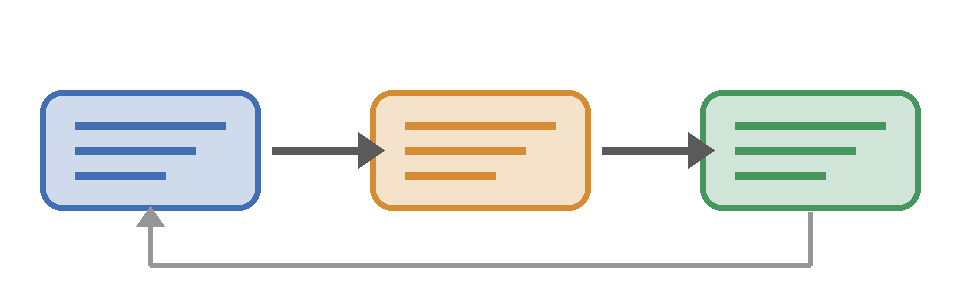
\includegraphics[width=0.9\linewidth]{../Images/overview.png}
\caption{The authoring loop: draft, proposal, decision. A kept proposal becomes a new revision, and the loop starts again.}
\label{fig:overview}
\end{figure}

Each kept change set, like each saved edit, becomes one revision in an append-only history~\cite{haber1991timestamp}.
Named versions mark milestones such as a submission, and draft branches hold changes that are not ready for the main line.
